\documentclass[12pt]{book}
\usepackage{amssymb,amsmath,latexsym,amsthm, hyperref, amsfonts, array, multicol}

\pagestyle{empty}

\newcommand{\longpage}{\enlargethispage*{1in}}

\usepackage{Sweave}
\begin{document}
\Sconcordance{concordance:PracticeSweave.tex:PracticeSweave.Rnw:%
1 7 1 1 0 2 1 1 5 16 1 1 8 10 0 1 2 3 1 1 2 5 0 1 2 4 1}



\begin{center}
\Large{Writing Functions in R}
\end{center}


\noindent Instead of copying and pasting commands over and over, the command ``function" will allow us to define functions that take arguments and return outputs such as graphs.


\noindent For example, instead of creating individual graphs for baby name trends over the years, we can define the function NameTrend to do this work for us. The format within an R chunk is 


\hfill\begin{minipage}{\dimexpr\textwidth-3cm}
 functionName <- function( arg1 = default1, arg2 = default2, ... ) \{Do stuff to the arguments here; the result of last line is returned, or we can use an explicit return() command.\}
\end{minipage}


\begin{Schunk}
\begin{Sinput}
> NameTrend <- function(names, gender) {
+   babynames %>% 
+   filter(name %in% names, sex == gender) %>%
+   ggplot() +
+   geom_line(aes(x = year, y = prop, color = name)) +
+     labs(x = "Year", y = "Proportion of Babies with This Name")
+ }
\end{Sinput}
\end{Schunk}


\noindent As we can see, NameTrend takes names and gender as arguments and returns a plot showing the trend of those names over time. For example,

\begin{Schunk}
\begin{Sinput}
> NameTrend(c("Nicole", "Rachelle"), "F")
\end{Sinput}
\end{Schunk}
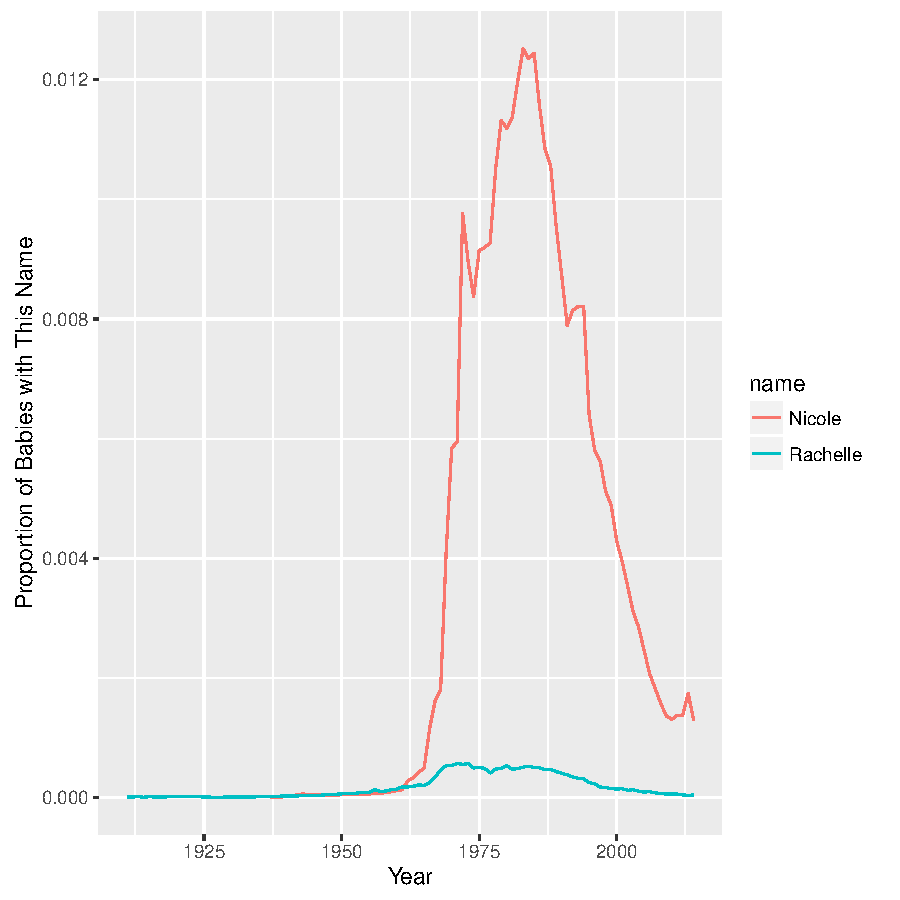
\includegraphics{PracticeSweave-003}


This has returned the graph for baby names Nicole (my sister) and Rachelle (me).

\end{document}
